\documentclass[letterpaper, 12pt]{article}
\usepackage{pgfplots}
\usepgfplotslibrary{fillbetween}
\pgfplotsset{compat=1.13}

\title{Principles of Microeconomics}
\author{Alvin Lin}
\date{August 2016 - December 2016}

\begin{document}

\maketitle

\tableofcontents

\section{Basics of Economics}
Economics is a social science that studies how people relate to each other in
a society. It studies how societies allocate scarce resources. If resources were
unlimited and freely available, the problem would be trivial.

\subsection{Fundamental Assumption}
The Fundamental Assumption in economics is that people face the problem
of scarcity. Scarcity arises when people have unlimited wants, but there are not
enough resources to satisfy those wants. Unlimited wants is not required for
a problem to arise, the problem exists when the total amount of a good desired
exceeds the total amount that is available.

\subsection{Rule of Thumb}
A good is scarce if whenever the price of it is zero there is not enough of it
provided to satisfy everyone's demand. Rarity is not the same as scarcity.

\subsection{The Fundamental Problem of Economics}
How \textit{do} societies deal with problems of scarcity?
\begin{itemize}
  \item We can find some answers by looking out into the world.
\end{itemize}
How \textit{should} societies deal with the problem of scarcity?
\begin{itemize}
  \item Should we train more nurses, or more lawyers?
  \item More food, or more weapons?
  \item Who gets the goods eventually?
  \item Should this be based on need or whether not the person can afford the
        good.
\end{itemize}
Scarcity involves tradeoffs. A society can invest more in education children,
or in national defense, but perhaps not both. A individual can fix her car, or
take a vacation, but not both.

\subsection{6 Key Ideas}
\begin{itemize}
  \item \textbf{Tradeoffs}: Individuals face tradeoffs when making choices.
  This is because of scarcity, something must be given up in order to get
  something else.
  \item \textbf{Benefits}: The benefit to a person of an activity is the most
  that a person is willing to give up in order to undertake that activity.
  \item \textbf{Costs}: The opportunity cost is what a person actually
  sacrifices when choosing one option over the other.
  \item \textbf{Choosing at the Margin}: Choosing at the margin involves
  the cost-benefit analysis of an activity to determine how much of it one
  should undertake.
  \item \textbf{People Make Rational Choices}: The idea that people make cold
  rational calculations is an assumption of our economics model.
  \item \textbf{Choices Respond to Incentives}: Individuals take into account
  costs and benefits when making choices.
\end{itemize}

\section{Model of an Economy}

\subsection{Production}
\textbf{The Economic Problem}: How are production decisions made?

\subsubsection{Production Possibilities Frontier (PPF)}
Determines the set of possible goods that can be produced at a given point in
time. It is the boundary between the combinations of goods that can be produced
and those that cannot be produced. The shape of the PPF curve is determined by
the resources available and the set of techniques available for producing
something. If you have a finite amount of a resource, your PPF will be
downwards sloping (true in almost all cases). Generally, the PPF is downwards
sloping and convex.

\subsubsection{Opportunity Cost (OC)}
The opportunity cost of an action is the highest valued alternative for
the action.

Example: If I value fruits in the following pattern:
\[ mango > orange > apple \]
\begin{itemize}
  \item My OC is mango if I choose apple.
  \item My OC is mango if I choose orange.
  \item My OC is orange if I choose mango.
\end{itemize}

\noindent\rule{13.7cm}{0.4pt}

Example: Two goods: grade on an economics exam (X), hours on a video game (Y),
6 hours available in total. The total cost of each hour spent on the game
is:
\begin{center}
  \begin{tabular}{|c|c|}
    \hline
    hours played & points lost \\ \hline
    0 & 0 \\ \hline
    1 & 2 \\ \hline
    2 & 15 \\ \hline
    3 & 30 \\ \hline
    4 & 50 \\ \hline
    5 & 75 \\ \hline
    6 & 100 \\ \hline
  \end{tabular}
\end{center}

The marginal cost of each hour is:
\begin{center}
  \begin{tabular}{|c|c|}
    \hline
    hours played & marginal cost \\ \hline
    1 & 2 \\ \hline
    2 & 13 \\ \hline
    3 & 15 \\ \hline
    4 & 20 \\ \hline
    5 & 25 \\ \hline
    6 & 25 \\ \hline
  \end{tabular}
\end{center}

The PPF is:
\begin{center}
  \begin{tabular}{|c|c|}
    \hline
    hours played & test grade \\ \hline
    0 & 100 \\ \hline
    1 & 98 \\ \hline
    2 & 85 \\ \hline
    3 & 70 \\ \hline
    4 & 50 \\ \hline
    5 & 25 \\ \hline
    6 & 0 \\ \hline
  \end{tabular}
\end{center}

\subsection{Decreasing Marginal Benefit}
The more of a good we have, the less we are willing to give up for one more
unit. The total benefit is always increasing, while the marginal benefit always
decreases (but is always greater than 0). If we are maximizing our benefit,
we need to find the allocation efficiency (total benefit - total cost).
\begin{center}
  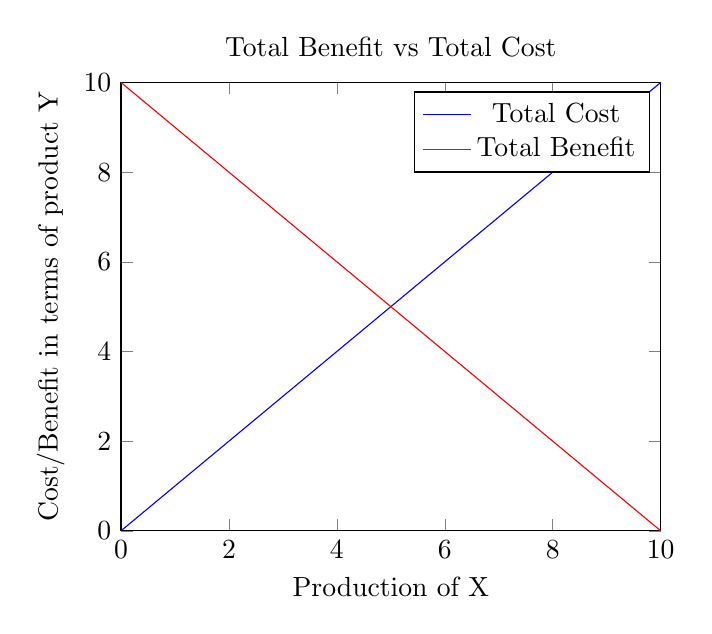
\begin{tikzpicture}
    \begin{axis} [
      title={Total Benefit vs Total Cost},
      xlabel={Production of X},
      ylabel={Cost/Benefit in terms of product Y},
      xmin=0, xmax=10,
      ymin=0, ymax=10
    ]
    \addplot[color=blue] coordinates { (0,0)(10,10) };
    \addlegendentry{Total Cost};
    \addplot[color=red] coordinates { (0,10)(10,0) };
    \addlegendentry{Total Benefit};
    \end{axis}
  \end{tikzpicture}
\end{center}
The allocation efficiency is maximized where the total cost and total benefit
meet.

\subsubsection{Practice Problem 1}
\begin{center}
  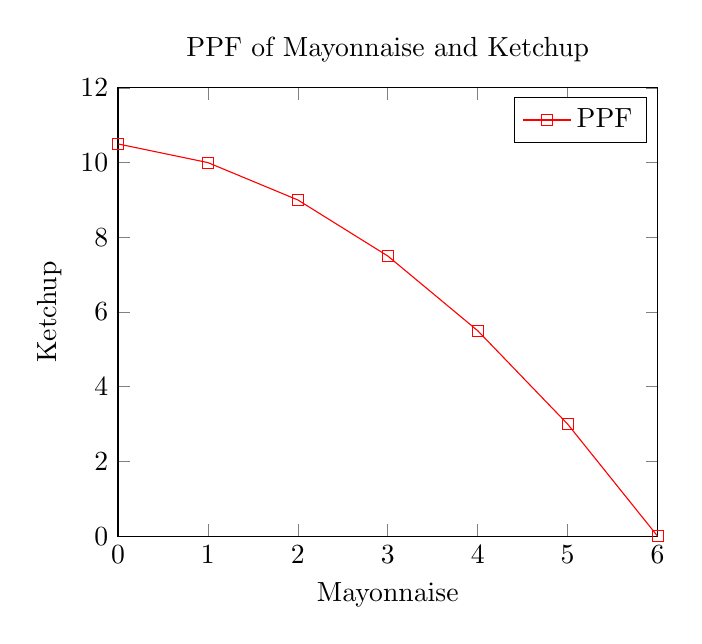
\begin{tikzpicture}
    \begin{axis} [
      title={PPF of Mayonnaise and Ketchup},
      xlabel={Mayonnaise},
      ylabel={Ketchup},
      xmin=0, xmax=6,
      ymin=0, ymax=12
    ]
    \addplot[color=red, mark=square] coordinates {
      (0,10.5)(1,10)(2,9)(3,7.5)(4,5.5)(5,3)(6,0)
    };
    \addlegendentry{PPF}
    \end{axis}
  \end{tikzpicture}
  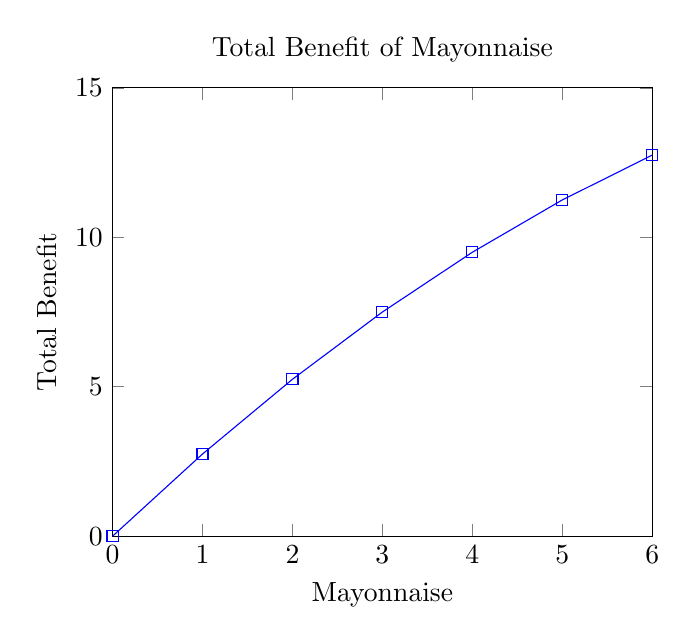
\begin{tikzpicture}
    \begin{axis} [
      title={Total Benefit of Mayonnaise},
      xlabel={Mayonnaise},
      ylabel={Total Benefit},
      xmin=0, xmax=6,
      ymin=0, ymax=15
    ]
    \addplot[color=blue, mark=square] coordinates {
      (0,0)(1,2.75)(2,5.25)(3,7.5)(4,9.5)(5,11.25)(6,12.75)
    };
    \end{axis}
  \end{tikzpicture}
\end{center}
What is the allocative efficient amounts of \( x_{1} \) and \( y \)?
\[ \mathrm{Allocative\ efficiency} = MC - MB \]
\begin{center}
  \begin{tabular}{|c|c|c|}
    \hline
    x & marginal cost & marginal benefit \\ \hline
    1 & 0.5  & 2.75 \\ \hline
    2 & 1    & 2.5  \\ \hline
    3 & 1.5  & 2.25 \\ \hline
    4 & 2    & 2    \\ \hline
    5 & 2.5  & 1.75 \\ \hline
    6 & 3    & 1.5  \\ \hline
  \end{tabular}
\end{center}
Producing 4 units of mayonnaise and 5.5 units of ketchup will maximize
production as well as benefit.

\subsubsection{Practice Problem 2}
Suppose you wake up one morning and discover that mayonnaise is good for your
health. What happens to allocative efficiency?
\begin{center}
  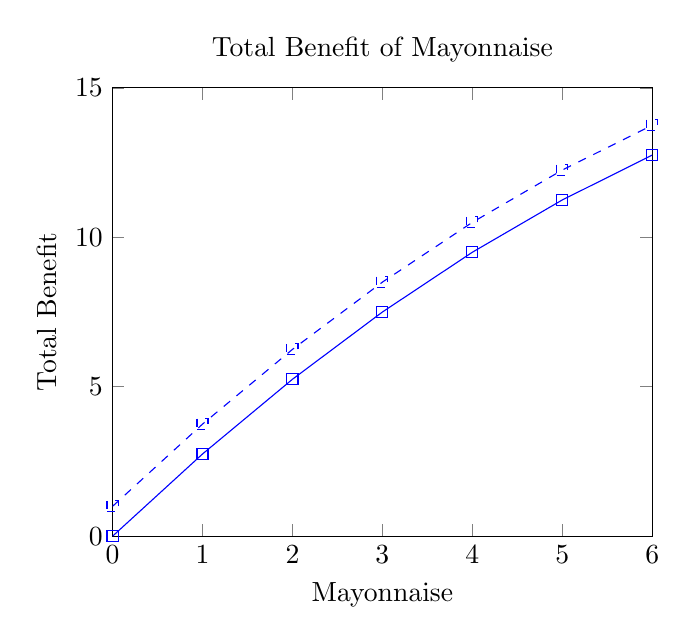
\begin{tikzpicture}
    \begin{axis} [
      title={Total Benefit of Mayonnaise},
      xlabel={Mayonnaise},
      ylabel={Total Benefit},
      xmin=0, xmax=6,
      ymin=0, ymax=15
    ]
      \addplot[color=blue, mark=square] coordinates {
        (0,0)(1,2.75)(2,5.25)(3,7.5)(4,9.5)(5,11.25)(6,12.75)
      };
      \addplot[color=blue, mark=square, dashed] coordinates {
        (0,1)(1,3.75)(2,6.25)(3,8.5)(4,10.5)(5,12.25)(6,13.75)
      };
    \end{axis}
  \end{tikzpicture}
\end{center}
The marginal benefit curve of mayonnaise will shift upwards, causing us to
consume more mayonnaise and less ketchup.

\subsubsection{Practice Problem 3}
Suppose it is a great season for your tomato garden. There are more resources
available to produce ketchup with. What happens to the marginal cost and
benefit of ketchup and mayonnaise?
\begin{center}
  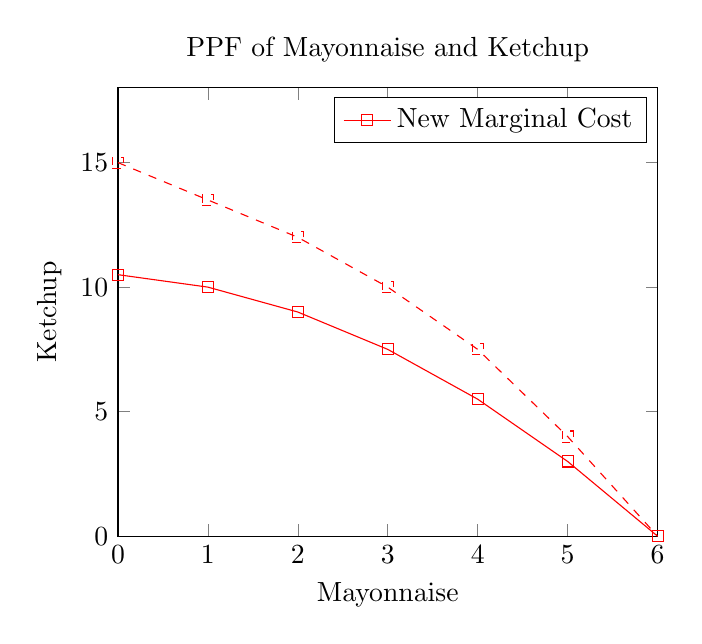
\begin{tikzpicture}
    \begin{axis} [
      title={PPF of Mayonnaise and Ketchup},
      xlabel={Mayonnaise},
      ylabel={Ketchup},
      xmin=0, xmax=6,
      ymin=0, ymax=18
    ]
    \addplot[color=red, mark=square] coordinates {
      (0,10.5)(1,10)(2,9)(3,7.5)(4,5.5)(5,3)(6,0)
    };
    \addplot[color=red, mark=square, dashed] coordinates {
      (0,15)(1,13.5)(2,12)(3,10)(4,7.5)(5,4)(6,0)
    };
    \addlegendentry{New Marginal Cost}
    \end{axis}
  \end{tikzpicture}
  \noindent\rule{13.7cm}{0.4pt}
  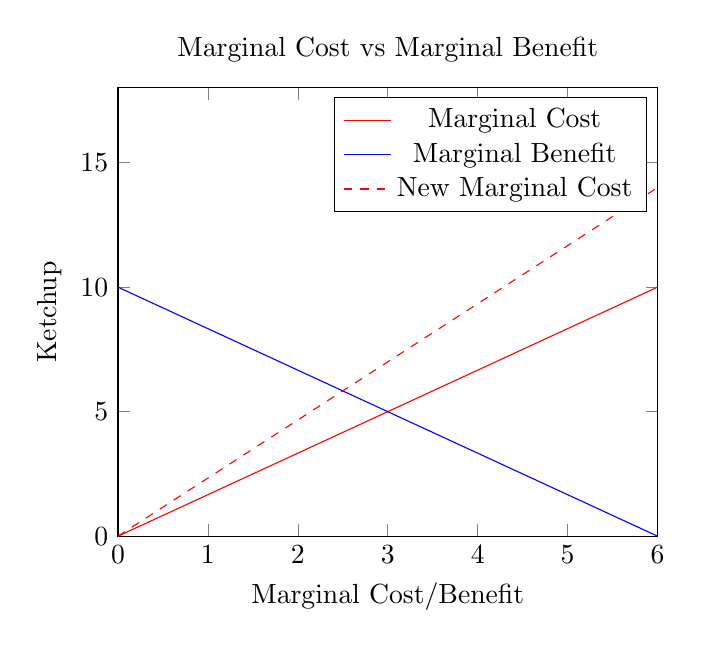
\begin{tikzpicture}
    \begin{axis} [
      title={Marginal Cost vs Marginal Benefit},
      xlabel={Marginal Cost/Benefit},
      ylabel={Ketchup},
      xmin=0, xmax=6,
      ymin=0, ymax=18
    ]
    \addplot[color=red] coordinates {
      (0,0)(6,10)
    };
    \addlegendentry{Marginal Cost}
    \addplot[color=blue] coordinates {
      (0,10)(6,0)
    };
    \addlegendentry{Marginal Benefit}
    \addplot[color=red, dashed] coordinates {
      (0,0)(6,14)
    };
    \addlegendentry{New Marginal Cost}
    \end{axis}
  \end{tikzpicture}
\end{center}
The marginal cost for ketchup will increase since you are able to produce more.
For each unit of mayonnaise you produce, you give up more ketchup that could
have been produced.

\subsection{Gains From Trade}
People could produce all the goods they consume on their own, or they could
specialize and conduct trade.
\newline
\textbf{Comparative Advantage (CA)}: A person (or country) has a comparative
advantage in an activity if they can perform that activity at a lower
opportunity cost that everyone else.
\newline
\textbf{Absolute Advantage (AA)}: A person (or country) has an absolute
advantage if they are more productive than others.
\begin{center}
  \begin{tabular}{|c|c|c|}
    \hline
    \multicolumn{3}{|c|}{Example 1} \\ \hline
           & Autos & Natural Gas  \\ \hline
    US     & 300 & 100            \\ \hline
    Canada & 60  & 80             \\ \hline
  \end{tabular}
\end{center}
In this example, the opportunity cost for Canada is \( \frac{3}{4} \) autos in
terms of natural gas, while the opportunity cost for the US is 3
autos in terms of natural gas. Therefore, Canada has a comparative advantage
in natural gas. Conversely, if this is the case, the the US must have a
comparative advantage in autos. \par
However, the US has an \textbf{absolute advantage} in natural gas and autos
since they produce more. \par
Whenever a country has a comparative advantage, it is always possible to
realize gains from trade.
\begin{center}
  \begin{tabular}{|c|c|c|}
    \hline
    \multicolumn{3}{|c|}{Example 2} \\ \hline
           & Autos & Natural Gas  \\ \hline
    US     & 150 & 50             \\ \hline
    Canada & 30  & 40             \\ \hline
    Totals & 180 & 90             \\ \hline
  \end{tabular}
\end{center}
If Canada were to shift more production to natural gas and the US were to shift
production to autos, then there would be a greater total of both.
\begin{center}
  \begin{tabular}{|c|c|c|}
    \hline
    \multicolumn{3}{|c|}{After Specializing} \\ \hline
           & Autos & Natural Gas  \\ \hline
    US     & 240 & 20             \\ \hline
    Canada & 0   & 80             \\ \hline
    Totals & 240 & 100            \\ \hline
  \end{tabular}
\end{center}

\section{Supply and Demand}
A market is any arrangement that enables buyers and sellers to get information
and do business with each other. One solution to the question of how scarce
resources should be allocated is the mechanism of a competitive market. \par
Markets have two parts, the \textbf{demand side}, which entails consumers
that way to buy, and the \textbf{supply side}, the sellers and producers.

\subsection{Demand}
You demand something if you want it, can afford it, and have definite plans to
buy it. The \textbf{quantity demanded} of a good or service is the amount that
consumers plan to buy during a particular time period at a particular price.

\subsubsection{The Law of Demand}
The Law of Demand states that, ceteris paribus, the higher the price
of a good, the smaller the quantity demanded. The lower the price of a good,
the larger the quantity desired. \textbf{Demand} refers to the entire
relationship between the price of a good and the quantity demanded of that
good. It is determined by preferences, income, and the price of other goods.
Two  factors for the Law of Demand are:

\paragraph{The Substitution Effect:}
When the price of a good increases, people seek substitutes for it, so the
quantity demanded decreases.

\paragraph{The Income Effect:}
When the price of a good increases relative to income, people cannot afford all
of the goods they could previously, so the quantity demanded of the good
decreases.

\subsubsection{The Demand Curve}
The demand curve shows the relationship between the quantity of a good and
its price when all other influences on a consumer's planned purchases remain
the same. It represents the willingness to pay for each quantity. The price
along the demand curve is the highest price a consumer is willing to pay
for that unit (Marginal Benefit Curve).

\subsection{Supply}
A firm supplies a good or service if it has the resources and technology to
produce that good, can make a profit from producing that good, and has
definite plans to produce and sell it. The \textbf{quantity supplied} of good
or service is the amount producers plan to sell during a particular time
period at a particular price. For any given price, the quantity supplied
tells us how much firms are willing to sell at that price.

\subsubsection{The Law of Supply}
The Law of Supply states that, ceteris paribus, producers are willing to supply
a good if they can at least cover their marginal costs. This results from the
general tendency for the marginal cost of producing a good to increase as the
quantity supplied increases.

\subsubsection{The Supply Curve and Supply Schedule}
The supply curve shows the relationship between the quantity supplied of a good
and its price when all other influences on a producer's plans remain the same.
Example supply curve:
\begin{center}
  \begin{tabular}{|c|c|}
    \hline
    Price of iPhones & Quantity Supplied (in thousands) \\ \hline
    0   & 0  \\ \hline
    150 & 10 \\ \hline
    300 & 20 \\ \hline
    450 & 30 \\ \hline
    600 & 40 \\ \hline
  \end{tabular}
\end{center}

\subsection{Market Equilibrium}
Equilibrium is a situation in which opposing forces balance each other. A
market equilibrium occurs when the price balances the plans of buyers and
sellers.

\subsubsection{Equilibrium Price \( P^{*} \)}
\[ Q_{S}\ at\ P^{*} = Q_{D}\ at\ P^{*} \]
The equilibrium price is the price at which the quantity demanded equals the
quanitity supplied. The equilibrium quantity is the quantity bought and sold
at that price. At prices below the equilibrium price there is excess demand,
or shortage. At prices above the equilibrium price there is excess supply,
or surplus. \par
At prices \textit{above} the equilibrium, a surplus forces prices down. At
prices \textit{below} the equilibrium, a shortage forces prices up. The
equilibrium point is stable, as there is no pressure on prices to change.

\subsubsection{Predicting Changes in Price and Quantity}
The demand curve shifts constantly. At the original price, there is either
a surplus or shortage. The price rises or falls to restore the equilibrium
and the quantity supplied moves along the supply curve. \par
The supply curve also shifts. At the original price, there can also be a
surplus or shortage. The price rises or falls to restore the equilibrium and
quantity demanded moves along the demand curve.

\subsubsection{Changes in Demand}
Changes in demand occur when factors other than the price influence buying
plans.

\paragraph{Prices of Related Goods:}
Prices of related goods can affect demand. A \textbf{substitute} is a good
that can be used in place of another good. A \textbf{complement} is a good
that is used in conjunction with another good.
\begin{itemize}
  \item A rise in the price of a substitute increases demand for the good.
  \item A decrease in the price of a substitute decreases demand for the good.
  \item A rise in the price of a complement decreases the demand for a good.
  \item A decrease in the price of a complement increases the demand for a good.
\end{itemize}

\paragraph{Expected Future Prices:}
Expected future prices also affect demand. If people expect the price to
increase in the future, they will demand more now. Conversely, if people
expect the price to decrease in the future, they will demand less now.

\paragraph{Income:}
For some goods, demand increases when income increases, but not all goods.
The demand of a \textbf{Normal Good} increases when income increases. The
demand of an \textbf{Inferior Good} decreases when income increases.

\paragraph{Expected Future Income and Credit:}
Demand can increase if people expect to earn more income in the future.

\paragraph{Population:} The larger the population is, the larger the demand is
for all goods.

\paragraph{Preferences:} If preferences change, demand will shift.

\subsubsection{Changes in Supply}
Changes in supply occur when any factor other than the price influences selling plans.

\paragraph{Prices of Factors of Production:}
If the price of a factor of production rises, the minimum price that a producer
is willing to accept for producing each quantity must also rise.

\paragraph{Prices of Related Goods:}
Prices of related goods can affect supply. A \textbf{subsitute in production}
is a good that can be produced using the same resources. A \textbf{complement
in production} is a good that must be produced in conjunction with another
good.
\begin{itemize}
  \item An increase in the price of a substitute in production increases the
        supply of a good.
  \item A decrease in the price of a substitute in production decreases the
        supply of a good.
  \item An increase in the price of a complement in production increases the
        supply of a good.
  \item A decrease in the price of a complement in production decreases the
        supply of a good.
\end{itemize}

\paragraph{Expected Future Prices:}
If the price of a good is expected to increase in the future, the supply of it
today decreases.

\paragraph{Number of Suppliers:}
The larger the number of suppliers of a good, the greater the supply is of the
good.

\paragraph{Technology:}
Advances in technology increase supply.

\paragraph{State of Nature:}
A natural disaster can decrease supply.

\section{Elasticity}
When supply decreases, the equilibrium price rises and the equilibrium
quantity decreases. The amount that the price and quantity increase and
decrease depends on the \textbf{responsiveness} of the quantity demanded of
a good to a change in its price.

\subsection{Price Elasticity of Demand}
One candidate for a measure of the responsiveness is the slope of the demand
curve. If the demand curve is flat, then the quantity decreases by a lot in
response to a relatively small increase in the price. If the demand curve is
steep, then the quantity decreases by a relatively small amount in response to
a relatively large increase in the price. Since the responsiveness depends on
the slope, we want a units free measurement when comparing it.
\[ E_{P} = \frac{\%\Delta Q}{\%\Delta P} \]
The elasticity in demand is equal to the percentage change in quantity demanded
over the percentage change in price.
\[ \%\Delta Q = \frac{Q_{new}-Q_{old}}{Q_{average}}\times 100 \]
\[ Q_{average} = \frac{Q_{new}+Q_{old}}{2} \]
\[ \%\Delta P = \frac{P_{new}-P_{old}}{P_{average}}\times 100 \]
\[ P_{average} = \frac{P_{new}+P_{old}}{2} \]
\[ E_{P} = \frac{\frac{Q_{new}-Q_{old}}{Q_{average}}\times 100}
            {\frac{P_{new}-P_{old}}{P_{average}}\times 100} = \]
\[ \frac{Q_{new}-Q_{old}}{P_{new}-P_{old}}\times
   \frac{P_{average}}{Q_{average}} \]
\[ \frac{Q_{new}-Q_{old}}{P_{new}-P_{old}}\times
   \frac{\frac{P_{new}+P_{old}}{2}}{\frac{Q_{new}+Q_{old}}{2}} \]
\[ \frac{Q_{new}-Q_{old}}{P_{new}-P_{old}}\times
   \frac{P_{new}+P_{old}}{Q_{new}+Q_{old}} \]

\subsubsection{Practice Problem}
Suppose you have been hired by the government to figure out a tax that will
reduce cigarette smoking by \( 25\% \). After a careful study, you decide
that the price elasticity of demand for cigarettes is \( E = -0.5 \). What
tax do you recommend to the government?
\[ E_{P} = -0.5 = \frac{\%\Delta Q}{\%\Delta P} = \frac{-25}{\%\Delta P} \]
\[ \%\Delta P = \frac{-25}{-0.5} = 50 \]
\begin{center}
  50\% tax on cigarettes.
\end{center}

\subsubsection{Ranges of Price Elasticity}
\begin{itemize}
  \item Elasticity can range from \( 0 \) to \( \infty \).
  \item Demand can be elastic (very responsive). \( |E_{P}| > 1 \)
  \item Demand can be inelastic (not very reponsive). \( |E_{P}| < 1 \)
  \item Demand can be unit elastic. \( |E_{P}| = 1 \)
\end{itemize}
\[ E_{P} \in \bigg(-\infty, -1\bigg): Elastic \]
\[ E_{P} \in \bigg(-1, 0\bigg]: Inelastic \]

\subsubsection{Practice Problem: \(|E| > 1 \)}
The percentage change in Q is greater than the percentage change in P.
For example, if the prices of movies increase from \$20 to \$30, and the demand
decreases from 1000 to 500.
\[ E_{P} = \frac{Q_{new}-Q_{old}}{P_{new}-P_{old}}\times
       \frac{P_{new}+P_{old}}{Q_{new}+Q_{old}} \]
\[ E_{P} = \frac{500-1000}{30-20}\times\frac{30+20}{500+1000} \]
\[ = \frac{-500}{10}\times\frac{50}{1500} = -\frac{5}{3} \]
\[ |E_{P}| = \frac{5}{3} \]

\subsubsection{Factors that Influence the Elasticity of Demand}
The elasticity of demand can change depending on different factors.

\paragraph{Closeness of Substitutes:} The demand for a good is elastic if a
substitute for it is easy to find. The demand for a good is inelastic if
substitutes are hard to find. \textbf{Necessitites}, such as food or housing,
generally have inelastic demand while \textbf{luxuries} generally have elastic
demand. The availability of substitutes depends on type of good and how
broadly or narrowly the good is defined.

\paragraph{The Proportion of Income Spent on the Good:}
The greater the proportion of income spent on the good, the greater the impact
of a price increase on the amount that people can afford. A higher proportion
spent on the good implies a more elastic demand.

\paragraph{Time Elapsed Since Price Change:}
More time elapsed implies more elastic demand.

\subsubsection{Price Elasticity Along a Linear Demand Curve}
\begin{center}
  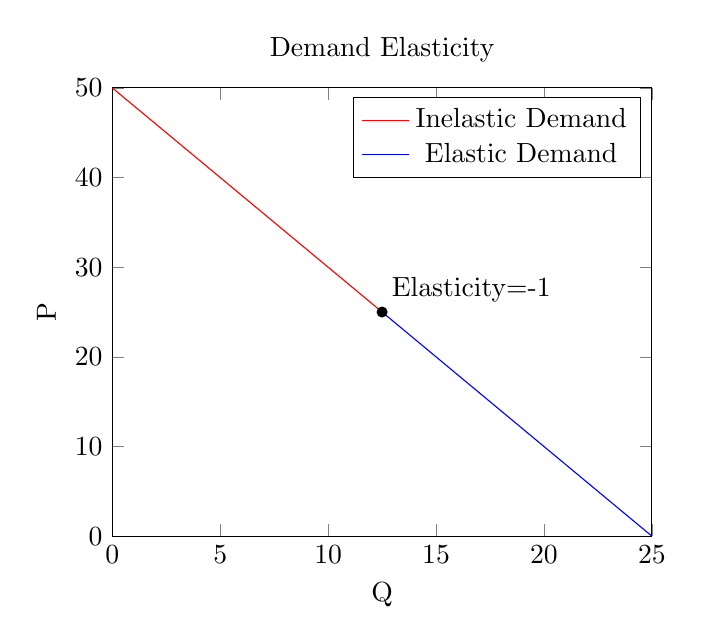
\begin{tikzpicture}
    \begin{axis} [
      title={Demand Elasticity},
      xlabel={Q},
      ylabel={P},
      xmin=0, xmax=25,
      ymin=0, ymax=50
    ]
      \addplot[color=red] coordinates { (0,50)(12.5,25) };
      \addlegendentry{Inelastic Demand}
      \addplot[color=blue] coordinates { (12.5,25)(25,0) };
      \addlegendentry{Elastic Demand}
      \fill (12.5,25) circle[radius=2pt];
      \draw (12.5,25) node[anchor=south west] {Elasticity=-1};
    \end{axis}
  \end{tikzpicture}
\end{center}

\subsubsection{Total Revenue and Elasticity}
A firm that sells a product obtains revenue from the sales. The total revenue
is the price of a good times the quantity sold.
\[ TR = P \times Q \]
If Starbucks sells a million lattes at \$4.00 each, then they make \$40,000,000
in total revenue. If they increase the price of lattes, then the quantity
demanded will go down.

\subsection{Income Elasticity of Demand}
Income elasticity is a measure of the responsiveness of the demand for a good to a change in income, ceteris paribus.
\[ E_{m} = \frac{\%\Delta Q}{\%\Delta M} \]
Like price elasticity of demand, this formula can be simplified to:
\[ E_{m} = \frac{Q_{new}-Q_{old}}{M_{new}-M_{old}}\times
           \frac{P_{new}+P_{old}}{Q_{new}+Q_{old}} \]

\subsubsection{Practice Problem 1}
Income rises from \$750 a week to \$1250 a week, while the quantity demanded
of Kraft Dinner decreases from 7 boxes a week to 3 boxes a week. What is the
elasticity?
\[ E_{m} = \frac{Q_{new}-Q_{old}}{M_{new}-M_{old}}\times
           \frac{M_{new}+M_{old}}{Q_{new}+Q_{old}} \]
\[ \frac{3-7}{1250-750}\times\frac{1250+750}{3+7} \]
\[ \frac{-4}{750}\times{2000}{10} \]
\[ = -\frac{8}{5} \]

\subsubsection{Practice Problem 2}
Income rises from \$750 a week to \$1250 a week, while the quantity demanded of
salmon fillet rises from 1 pound a week to 2 pounds a week. What is the
elasticity?
\[ E_{m} = \frac{Q_{new}-Q_{old}}{M_{new}-M_{old}}\times
           \frac{M_{new}+M_{old}}{Q_{new}+Q_{old}} \]
\[ \frac{2-1}{1250-750}\times\frac{1250+750}{2+1} \]
\[ \frac{1}{500}\times\frac{2000}{3} \]
\[ = \frac{4}{3} \]

\subsubsection{Ranges of Income Elasticity}
If income elasticity is position and greater than one, it is income elastic.
If income elasticity is negative and less than minus one, it is income elastic.
\textit{A one percent increase in income results in a greater than one percent
increase in quantity demanded}. \par
An income elasticity between -1 and 1 means the it is income inelastic.

\subsection{Cross Price Elasticity of Demand}
Cross elasticity is a measure of the responsiveness of the demand for a good
to changes in the price of a \textit{substitute} or \textit{complement},
ceteris paribus.
\[ E_{X,Y} = \frac{\%\Delta Q_{X}}{\%\Delta P_{Y}} \]
\[ E_{X,Y} = \frac{Q_{X}^{new}-Q_{x}^{old}}{P_{Y}^{new}-P_{Y}^{old}}\times
             \frac{P_{Y}^{new}+P_{Y}^{old}}{Q_{X}^{new}+Q_{x}^{old}} \]

\subsubsection{Practice Problem}
When the price of Adidas increases from \$100 to \$120, the quantity demanded
of Nikes increases from 1 million to 3 million per year.
\[ E_{X,Y} = \frac{3-1}{120-100}\times\frac{120+100}{3+1} \]
\[ \frac{2}{20}\times\frac{220}{4} \]
\[ = \frac{11}{2} \]

\subsubsection{Ranges of Cross Price Elasticity}
The magnitude of the elasticity indicates how closely related the goods are.
A large positive elasticity indicates the goods are closely related substitutes.
A small positive elasticity indicates they are substitutes but not closely
related. A small negative elasticity indicates they are complements but not
closely related and a large negative elasticity indicates they are close
complements.
\begin{center}
  \begin{tabular}{|c|c|c|}
    \hline
    Sign & Magnitude & \\ \hline
    -    & large     & close complements\\ \hline
    -    & small     & complements \\ \hline
    +    & large     & close substitutes \\ \hline
    +    & small     & substitutes \\ \hline
    0    & 0         & not related \\ \hline
  \end{tabular}
\end{center}

\subsection{Elasticity of Supply}
Elasticity of Supply is a measure of the responsiveness of the quantity supplied
of a good to changes in the price of the good, ceteris paribus. The formula
follows the same form, but \( Q \) is now a quantity of supply instead of a
quantity of demand.
\[ E_{S} = \frac{\%\Delta Q}{\%\Delta P} \]
\[ E_{S} = \frac{Q_{new}-Q_{old}}{P_{new}-P_{old}}\times
           \frac{P_{new}+P_{old}}{Q_{new}+Q_{old}} \]

\subsubsection{Ranges of Elasticity of Supply}
\begin{itemize}
  \item Supply is perfectly inelastic. \( E_{S} = 0 \)
  \item Supply is inelastic. \( E_{S} \in (1, 1) \)
  \item Supply is unit elastic. \( E_{S} = 1 \)
  \item Supply is elastic. \( E_{S} \in (1, \infty) \)
  \item Supply is perfectly elastic. \( E_{S} = \infty \)
\end{itemize}

\subsubsection{Factors that Influence the Elasticity of Supply}
The elasticity of supply can change depending on different factors.

\paragraph{Resource Substitution Possibility:}
Some goods can only be produced using rare resources. These have inelastic
supply curves. Other goods are produced using resources that can be used in
a wide variety of production tasks.

\paragraph{Time Frame for the Supply Decision:}
Short run supply determines the changes to supply that can occur when some of
the factors of production remain fixed. A firm can layoff or hire new workers
in the short run. But it may not be able to build a larger factory. Long run
supply determines the changes in supply that are possible when all factors are
variable.

\subsubsection{Elasticity Along a Linear Supply Curve}
\[ E_{S} = \frac{1}{slope}\times\frac{P_{average}}{Q_{average}} \]
\begin{center}
  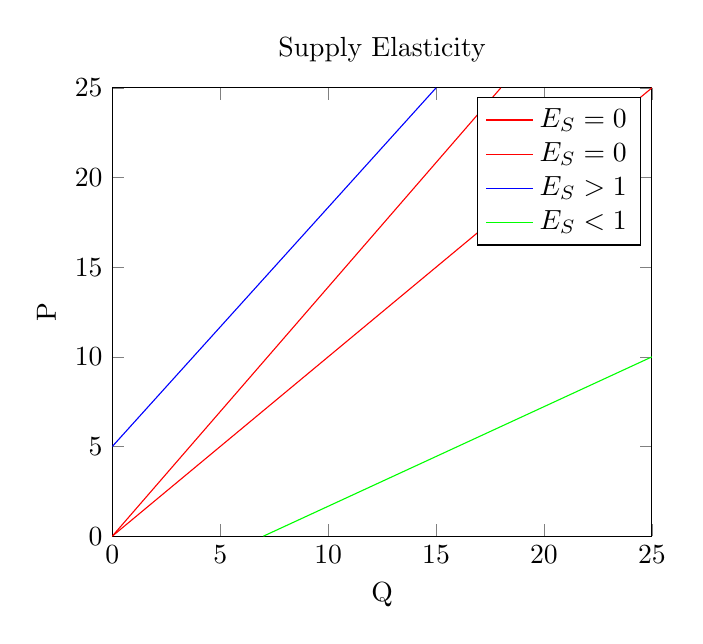
\begin{tikzpicture}
    \begin{axis} [
      title={Supply Elasticity},
      xlabel={Q},
      ylabel={P},
      xmin=0, xmax=25,
      ymin=0, ymax=25
    ]
      \addplot[color=red] coordinates { (0,0)(25,25) };
      \addlegendentry{\( E_{S} = 0 \)}
      \addplot[color=red] coordinates { (0,0)(18,25) };
      \addlegendentry{\( E_{S} = 0 \)}
      \addplot[color=blue] coordinates { (0,5)(15,25) };
      \addlegendentry{\( E_{S} > 1 \)}
      \addplot[color=green] coordinates { (7,0)(25,10) };
      \addlegendentry{\( E_{S} < 1 \)}
    \end{axis}
  \end{tikzpicture}
\end{center}
Any supply curve that passes through the origin has an elasticity of 1.

\section{Efficiency and Equity}
How are goods allocated efficiently? How are goods allocated fairly? A
\textbf{normative statement} is an expression of how things ought to be, and a
\textbf{positive statement} is an expression of how things are.

\subsection{Competitive Market}
Trade occurs at the equilibrium price. Every buyer willing to pay that price
or more gets to buy. Every seller willing to trade at that price or less
gets to sell. A competitive market has no external control. Many individuals
acting in their own self interest determines how resources are allocated.

\subsection{Consumer Surplus}
Consumer surplus is the excess of the benefit received from a good over the
amount paid for it.
\[ \mathrm{consumer\ surplus} = \mathrm{marginal\ benefit}-
   \mathrm{the\ price\ paid} \]

\subsubsection{Example}
Suppose I am willing to pay \$5 for the first cheeseburger and \$4 for the
second but I purchase 2 cheeseburgers at \$3 each. My marginal benefit for the
first cheeseburger was \$5 and my marginal benefit for the second was \$4. The
surplus for the first cheeseburger was \$2 and the surplus for the second
cheeseburger was \$1. The consumer surplus obtained is \$3.

\subsection{Benefit, Cost, and Surplus}
The \textit{marginal benefit} is the value to a person of one more good or
service. We can measure this as the maximum price that a person is willing to
pay for one more unit of a good. An individual's demand curve is their marginal
benefit curve. \textbf{For any individual, the consumer surplus from consuming
q units is the area below the individual's demand curve above the price, up to
q}. \par
\textbf{Individual Demand} is the relationship between the price of a good and
the quantity demanded by a particular individual. \par
\textbf{Market Demand} is the relationship between the price of a good and the
quantity demanded by all the buyers in a market, derived by summing all the
individual quantities demanded at each price.

\subsubsection{Example}
\begin{center}
  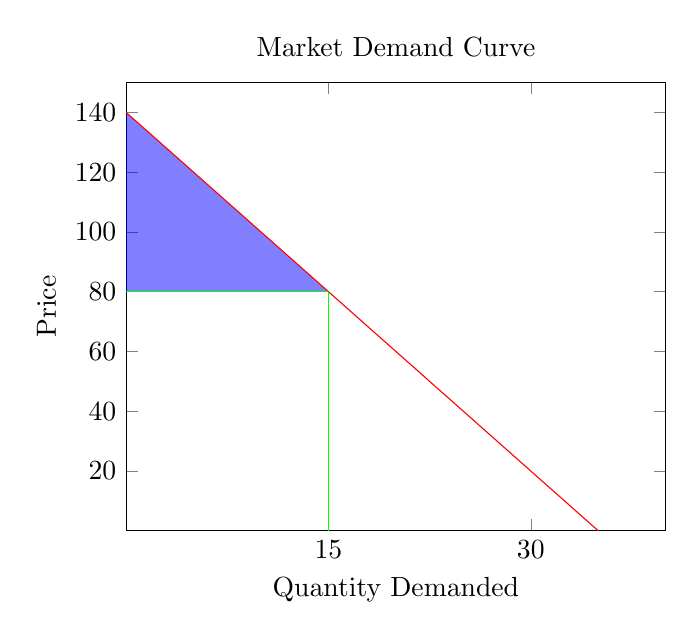
\begin{tikzpicture}
    \begin{axis} [
      title={Market Demand Curve},
      xlabel={Quantity Demanded},
      ylabel={Price},
      xmin=0, xmax=40,
      ymin=0, ymax=150,
      ytick={20,40,60,80,100,120,140},
      xtick={15,30,45}
    ]
    \addplot[name path=path, color=red] coordinates { (0,140) (35,0) };
    \addplot[name path=bound, color=green] coordinates { (0,80) (15,80) };
    \addplot[color=green] coordinates { (15,80)(15,0) };
    \addplot[color=blue, fill=blue, fill opacity=0.5]
      fill between[of=path and bound, soft clip={domain=0:15}];
    \end{axis}
  \end{tikzpicture}
\end{center}
The consumer surplus when price is 80 is the area under the curve above 80.
\[ A = \frac{1}{2}bh = \frac{1}{2}\times15\times60 = 450 \]

\subsection{Producer Surplus}
Producer surplus is the excess of the revenue received from a good over the
amount paid to produce it.
\[ \mathrm{producer\ surplus} = \mathrm{total\ revenue}-\mathrm{total\ cost} \]
Given a price, a supplier will supply the quantity that makes profit (producer
surplus) as large as possible. A producer maximimizes producer surplus (profit)
by choosing the quantity that sets \( P = MC \).

\subsubsection{Market Supply}
Market supply gives tne relationship between price and quantity supplied by the
whole market. It is derived by summing all the \textit{individual quantities
supplied} at each price.

\subsubsection{Market Producer Surplus}
Market producer surplus is the sum of all the individual producer surpluses. It
is calculuated as the area above the market supply function but below the market
price. Given a price, a consumer will demand the quantity that makes her
consumer surplus as large as possible. \par
The quantity supplied is determined by each individual producer supplying the
amount that maximizes her profits. The quantity demanded is determined by each
individual consumer demanding the amount that maximizes his consumer surplus.

\subsubsection{Total Surplus}
The total surplus is the total benefit to society net of all costs.
\[ \mathrm{total\ surplus} = \mathrm{producer\ surplus\ }(PS)+
   \mathrm{consumer\ surplus\ }(CS) \]
Total surplus is maximized in a competitive equilibrium.
\begin{center}
  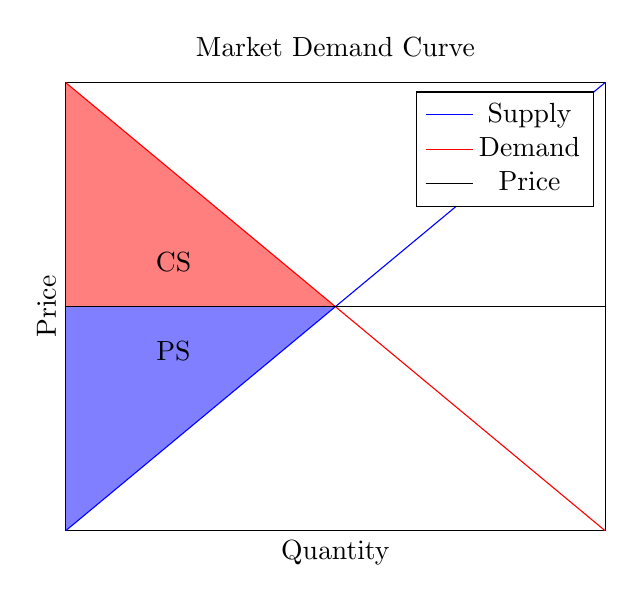
\begin{tikzpicture}
    \begin{axis} [
      title={Market Demand Curve},
      xlabel={Quantity},
      ylabel={Price},
      xtick=\empty,
      ytick=\empty,
      xmin=0, xmax=100,
      ymin=0, ymax=100
    ]
      \addplot[name path=supply, color=blue] coordinates { (0,0) (100,100) };
      \addlegendentry{Supply};
      \addplot[name path=demand, color=red] coordinates { (0,100) (100,0) };
      \addlegendentry{Demand};
      \addplot[name path=split, color=black] coordinates { (0,50) (100,50) };
      \addlegendentry{Price};
      \addplot[color=blue, fill=blue, fill opacity=0.5]
        fill between [of=split and supply, soft clip={domain=0:50}];
      \addplot[color=red, fill=red, fill opacity=0.5]
        fill between [of=split and demand, soft clip={domain=0:50}];
      \node[draw=none] at (20,60) {CS};
      \node[draw=none] at (20,40) {PS};
    \end{axis}
  \end{tikzpicture}
\end{center}

\subsection{Market Failure}
When there is a fixed price imposed on a good, there can be different
effects on consumers and producers.
\begin{center}
  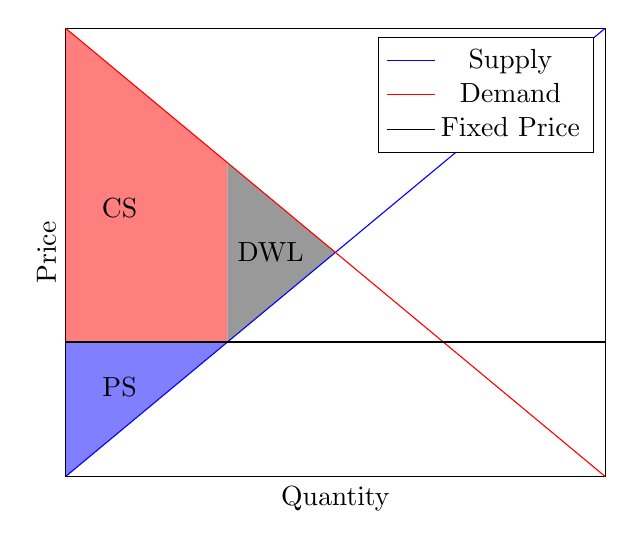
\begin{tikzpicture}
    \begin{axis} [
      xlabel={Quantity},
      ylabel={Price},
      xtick=\empty,
      ytick=\empty,
      xmin=0, xmax=100,
      ymin=0, ymax=100
    ]
      \addplot[name path=supply, color=blue] coordinates { (0,0) (100,100) };
      \addlegendentry{Supply};
      \addplot[name path=demand, color=red] coordinates { (0,100) (100,0) };
      \addlegendentry{Demand};
      \addplot[name path=split, color=black] coordinates { (0,30) (100,30) };
      \addlegendentry{Fixed Price};
      \addplot[color=blue, fill=blue, fill opacity=0.5]
        fill between [of=split and supply, soft clip={domain=0:30}];
      \addplot[color=red, fill=red, fill opacity=0.5]
        fill between [of=split and demand, soft clip={domain=0:30}];
      \addplot[color=black, fill=black!40]
        fill between [of=supply and demand, soft clip={domain=30:50}];
      \node[draw=none] at (10,60) {CS};
      \node[draw=none] at (10,20) {PS};
      \node[draw=none] at (38,50) {DWL};
    \end{axis}
  \end{tikzpicture}
  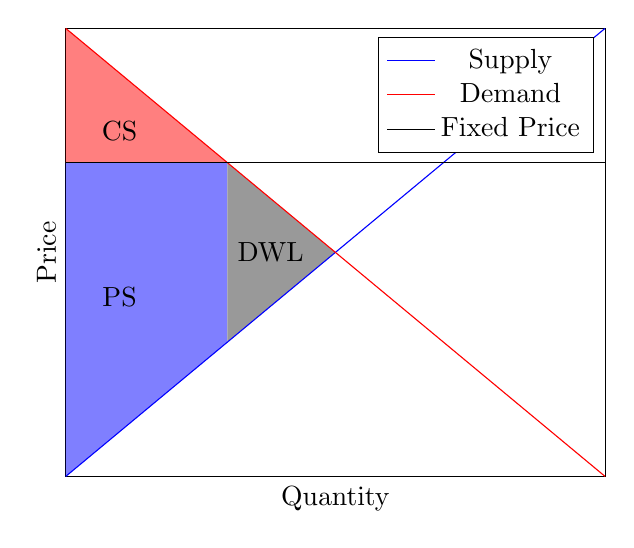
\begin{tikzpicture}
    \begin{axis} [
      xlabel={Quantity},
      ylabel={Price},
      xtick=\empty,
      ytick=\empty,
      xmin=0, xmax=100,
      ymin=0, ymax=100
    ]
      \addplot[name path=supply, color=blue] coordinates { (0,0) (100,100) };
      \addlegendentry{Supply};
      \addplot[name path=demand, color=red] coordinates { (0,100) (100,0) };
      \addlegendentry{Demand};
      \addplot[name path=split, color=black] coordinates { (0,70) (100,70) };
      \addlegendentry{Fixed Price};
      \addplot[color=blue, fill=blue, fill opacity=0.5]
        fill between [of=split and supply, soft clip={domain=0:30}];
      \addplot[color=red, fill=red, fill opacity=0.5]
        fill between [of=split and demand, soft clip={domain=0:30}];
      \addplot[color=black, fill=black!40]
        fill between [of=supply and demand, soft clip={domain=30:50}];
      \node[draw=none] at (10,77) {CS};
      \node[draw=none] at (10,40) {PS};
      \node[draw=none] at (38,50) {DWL};
    \end{axis}
  \end{tikzpicture}
\end{center}
The triangle of surplus lost is called dead-weight loss (DWL). It represents
the decrease in total surplus resulting from an inefficient level of production.
This is a situation called market failure where a market fails to achieve an
efficient outcome and happens because of overproduction or underproduction. \par
Amount of trade can also affect dead-weight loss. Let \( TS* \) be the optimal
total surplus at the competitive equilibrium quantity \( Q* \). If the quantity
traded is \( \neq Q* \), then \( TS < TS* \).
\begin{center}
  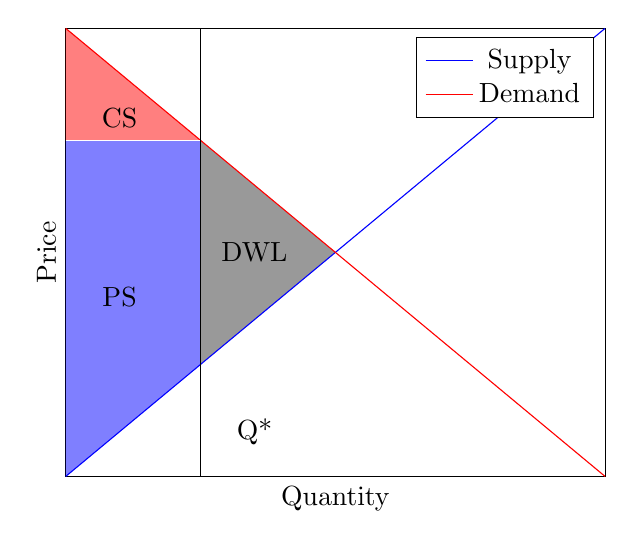
\begin{tikzpicture}
    \begin{axis} [
      xlabel={Quantity},
      ylabel={Price},
      xtick=\empty,
      ytick=\empty,
      xmin=0, xmax=100,
      ymin=0, ymax=100
    ]
      \addplot[name path=supply, color=blue] coordinates { (0,0) (100,100) };
      \addlegendentry{Supply};
      \addplot[name path=demand, color=red] coordinates { (0,100) (100,0) };
      \addlegendentry{Demand};
      \addplot[name path=split, color=white] coordinates { (0,75) (25,75) };
      \addplot[name path=q, color=black] coordinates { (25,0) (25,100) };
      \addplot[color=blue, fill=blue, fill opacity=0.5]
        fill between [of=split and supply, soft clip={domain=0:25}];
      \addplot[color=red, fill=red, fill opacity=0.5]
        fill between [of=split and demand, soft clip={domain=0:25}];
      \addplot[color=black, fill=black!40]
        fill between [of=supply and demand, soft clip={domain=25:50}];
      \node[draw=none] at (10,80) {CS};
      \node[draw=none] at (10,40) {PS};
      \node[draw=none] at (35,50) {DWL};
      \node[draw=none] at (35,10) {Q*};
    \end{axis}
  \end{tikzpicture}
\end{center}

\subsubsection{Sources of Market Failure}

\paragraph{Price and Quantity Regulation:}
Price regulations such as rent control or minimum wage or quantity regulations
such as quotas can cause market failure.

\paragraph{Taxes and Subsidies:}
Taxes and subsidies can incentivize or deincentivize production of a good.

\paragraph{Externalities:}
An externality is a cost or benefit to someone other than the seller or buyer.
If the externality imposes a cost on an outside party, then there is
overproduction relative to what is socially optimal. If the externality provides
a benefit to an outside party, then there is underproduction relative to what is
socially optimal.

\paragraph{Public Goods and Common Resources:}
A public good is a good with usage that cannot be regulated and that can be
consumed by many persons simultaneously, such as national defense and clean air.
Common resources are resources owned by no particular individual but available
to everyone.

\paragraph{Monopoly:}
A monopoly is a firm that is the sole supplier of a good or service.

\paragraph{High Transaction Costs:}
Transaction costs are the costs required for the market to operate.

\section{Governments and Markets}

\subsection{Price Ceilings}
A \textbf{price ceiling} is a regulation making it illegal to charge more than
specified price. A price ceiling set above the equilibrium price has no effect.
A price ceiling set below the equilibrium price results in dead-weight loss.

\subsubsection{Consequences of a Binding Price Ceiling}
\begin{itemize}
  \item Shortage
  \item A transfer of surplus from producers to consumers
  \item Deadweight loss
  \item Producer surplus decreases
  \item Consumer surplus increases
\end{itemize}

\subsubsection{Rent Ceilings}
A \textbf{rent ceiling} is a government regulation making it illegal to charge
a rent higher than a specified level. Landlords will restrict the supply in
response while the quantity demanded increases. This causes a housing shortage,
dead-weight loss, and a transfer of surplus from landlords to renters. The
opportunity costs to renters increases since finding an apartment requires more
search.

\subsubsection{Consequences of Rent Ceilings}
The rent ceiling encourages an illegal market for apartments. Renters and
landlords figure out ways to increase the rents. Landlords introduce
``additional service'' charges and engage in side deals. The effects of black
market activities is determined by how strictly enforced rent control is.
If the control is lax, the black market price is very close to the market price.
If the control is strict, the black market price is much higher than the market
price.

\subsubsection{Example}
\begin{center}
  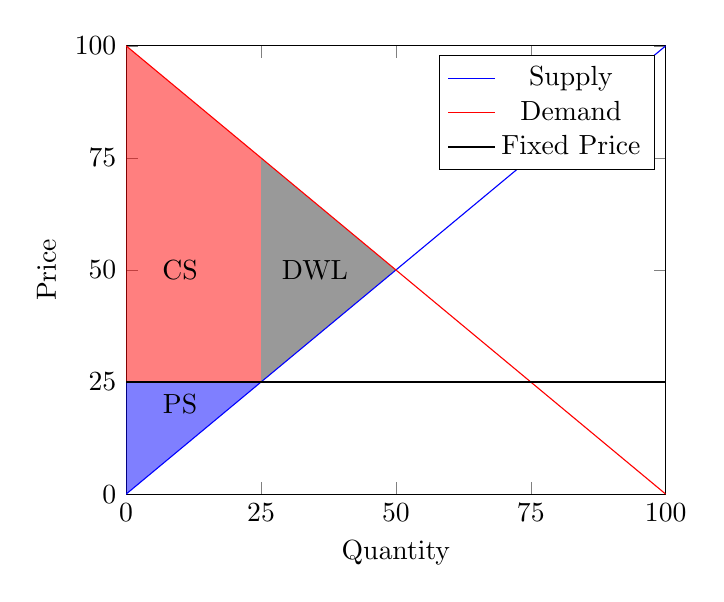
\begin{tikzpicture}
    \begin{axis} [
      xlabel={Quantity},
      ylabel={Price},
      xtick={0,25,50,75,100},
      ytick={0,25,50,75,100},
      xmin=0, xmax=100,
      ymin=0, ymax=100
    ]
      \addplot[name path=supply, color=blue] coordinates { (0,0) (100,100) };
      \addlegendentry{Supply};
      \addplot[name path=demand, color=red] coordinates { (0,100) (100,0) };
      \addlegendentry{Demand};
      \addplot[name path=split, color=black] coordinates { (0,25) (100,25) };
      \addlegendentry{Fixed Price};
      \addplot[color=blue, fill=blue, fill opacity=0.5]
        fill between [of=split and supply, soft clip={domain=0:25}];
      \addplot[color=red, fill=red, fill opacity=0.5]
        fill between [of=split and demand, soft clip={domain=0:25}];
      \addplot[color=black, fill=black!40]
        fill between [of=supply and demand, soft clip={domain=25:50}];
      \node[draw=none] at (10,50) {CS};
      \node[draw=none] at (10,20) {PS};
      \node[draw=none] at (35,50) {DWL};
    \end{axis}
  \end{tikzpicture}
\end{center}
At the equilibrium price, there was no dead-weight loss, with the consumer
and producer surplus equal to 1250. At a fixed price of 25, there is align
dead-weight loss of 625. The new consumer surplus is 1562.5. The new
producer surplus is 312.5. The total surplus is 1875.
\[ \Delta CS = +312.5 \]
\[ \Delta PS = -937.5 \]
\[ \Delta TS = -625 \]

\subsection{Price Floors}
A \textbf{price floor} is a regulation making it illegal to charge less than a
specified price. A price floor set below the equilibrium price has no effect.
A price floor set above the equilibrium price results in dead-weight loss.

\subsubsection{Consequences of a Binding Price Floor}
\begin{itemize}
  \item Surplus
  \item A transfer of surplus from consumers to producers
  \item Deadweight loss
  \item Consumer surplus decreases
  \item Producer surplus increases
\end{itemize}

\subsubsection{Minimum Wage}
\textbf{Minimum wage} is a government regulation making it illegal to pay a
worker less than a specified wage. It is a price floor imposed on the labor
market. The labor market has a supply of labor (workers), and demand for labor
(producers of goods and services).

\subsubsection{Consequences of a Minimum Wage}
\begin{itemize}
  \item Unemployment
  \item Deadweight loss
  \item A transfer of surplus from employees to workers
  \item Consumer surplus decreases
  \item Producer surplus increases or decreases
  \item Benefits workers that keep their jobs
  \item Hurts people that are looking for work and those that lose their jobs
\end{itemize}

\subsubsection{Example}
\[ Supply: P = 1+Q \]
\[ Demand: P = 16-2Q \]
\[ S = D \]
\[ 1+Q^{*} = 16-2Q^{*} \]
\[ 3Q^{*} = 15 \]
\[ Q^{*} = 5 \]
\begin{center}
  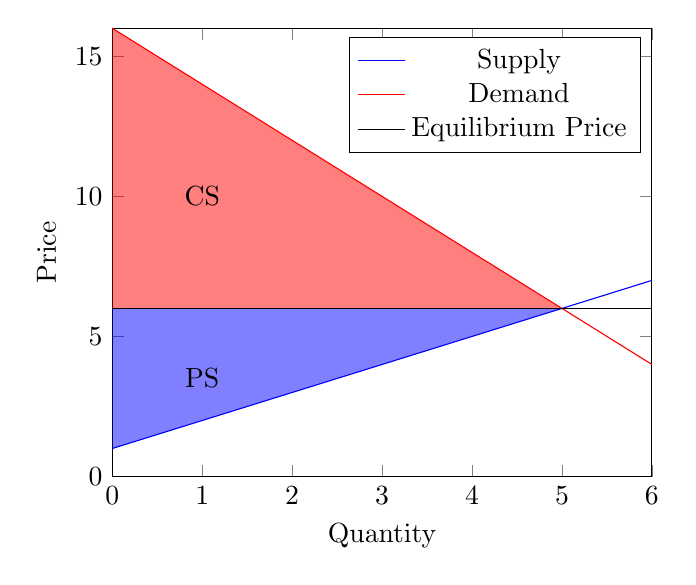
\begin{tikzpicture}
    \begin{axis} [
      xlabel={Quantity},
      ylabel={Price},
      xmin=0, xmax=6,
      ymin=0, ymax=16
    ]
      \addplot[name path=supply, color=blue] coordinates { (0,1) (6,7) };
      \addlegendentry{Supply};
      \addplot[name path=demand, color=red] coordinates { (0,16) (6,4) };
      \addlegendentry{Demand};
      \addplot[name path=split, color=black] coordinates { (0,6) (6,6) };
      \addlegendentry{Equilibrium Price};
      \addplot[color=blue, fill=blue, fill opacity=0.5]
        fill between [of=split and supply, soft clip={domain=0:5}];
      \addplot[color=red, fill=red, fill opacity=0.5]
        fill between [of=split and demand, soft clip={domain=0:5}];
      \node[draw=none] at (1,10) {CS};
      \node[draw=none] at (1,3.5) {PS};
    \end{axis}
  \end{tikzpicture}
\end{center}
At \( Q^{*} \):
\[ PS = \frac{1}{2}bh = \frac{1}{2}(5)(5) = 12.5 \]
\[ CS = \frac{1}{2}bh = \frac{1}{2}(10)(5) = 25 \]
\[ TS = 37.5 \]
What is the effect of a minimum wage of \$10 on consumer surplus, producer
surplus, and total surplus?
\begin{center}
  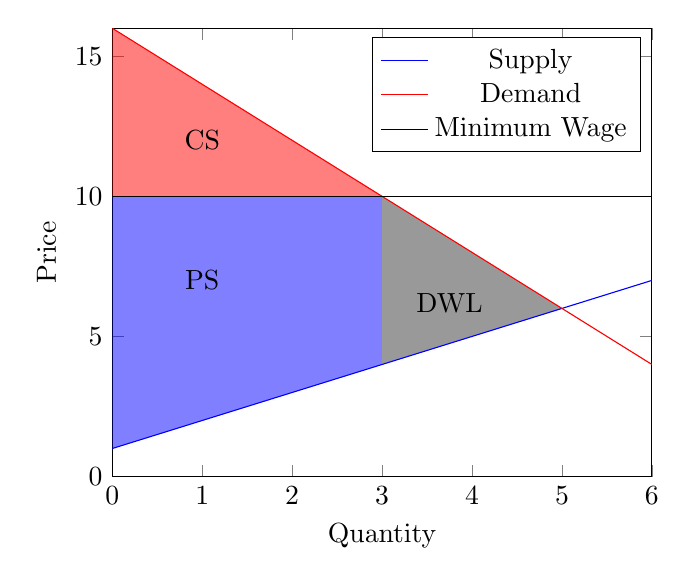
\begin{tikzpicture}
    \begin{axis} [
      xlabel={Quantity},
      ylabel={Price},
      xmin=0, xmax=6,
      ymin=0, ymax=16
    ]
      \addplot[name path=supply, color=blue] coordinates { (0,1) (6,7) };
      \addlegendentry{Supply};
      \addplot[name path=demand, color=red] coordinates { (0,16) (6,4) };
      \addlegendentry{Demand};
      \addplot[name path=split, color=black] coordinates { (0,10) (6,10) };
      \addlegendentry{Minimum Wage};
      \addplot[color=blue, fill=blue, fill opacity=0.5]
        fill between [of=split and supply, soft clip={domain=0:3}];
      \addplot[color=red, fill=red, fill opacity=0.5]
        fill between [of=split and demand, soft clip={domain=0:3}];
      \addplot[color=black, fill=black!40]
        fill between [of=supply and demand, soft clip={domain=3:5}];
      \node[draw=none] at (1,12) {CS};
      \node[draw=none] at (1,7) {PS};
      \node[draw=none] at (3.75,6.2) {DWL};
    \end{axis}
  \end{tikzpicture}
\end{center}
At the fixed minimum wage:
\[ PS = \frac{1}{2}(b_{1}+b_{2})h = \frac{1}{2}(9+6)(3) = 22.5 \]
\[ CS = \frac{1}{2}bh = \frac{1}{2}(3)(6) = 9 \]
\[ TS = 31.5 \]
Change:
\[ \Delta PS = 10 \]
\[ \Delta CS = -16 \]
\[ \Delta TS = -6 \]

\subsection{Taxes}
A tax a levy imposed on an individual or other legal entity by the state.
Failure to pay is punishable by law. In the market, a tax on sellers is a fixed
fee per unit sold. A tax on buyers is a fixed fee for each unit purchased. \par
Other taxes include taxes on trade, proportional taxes on expenditure or
revenue, estate taxes, gift taxes, and fixed flat taxes.

\subsubsection{Key Questions}
\begin{itemize}
  \item How much tax revenue is raised?
  \item Does the tax result in an inefficient quantity traded?
  \item Who bears the burden of the tax?
  \item What are the effects on producer surplus, consumer surplus, and total
  surplus.
\end{itemize}

\subsubsection{Tax Incidence}
\textbf{Tax Incidence} is the division of the burden of a tax between buyers
and sellers. If a tax is imposed on the sale of a good, the price faced by
consumers might increase by the whole amount, part of it, or by nothing at all.
If the price does not change, then the cost of the tax is borne by sellers. \par
It does not matter whether the consumer or the producer is taxed.

\subsubsection{Consequences of Taxes}
\begin{itemize}
  \item Increases in the price
  \item Decrease in quantity traded
  \item Producer surplus and consumer surplus decrease
  \item Deadweight loss
  \item Tax revenue raised by the government
\end{itemize}

\subsubsection{Example}
Suppose the government imposes a \$2 tax on sellers:
\begin{center}
  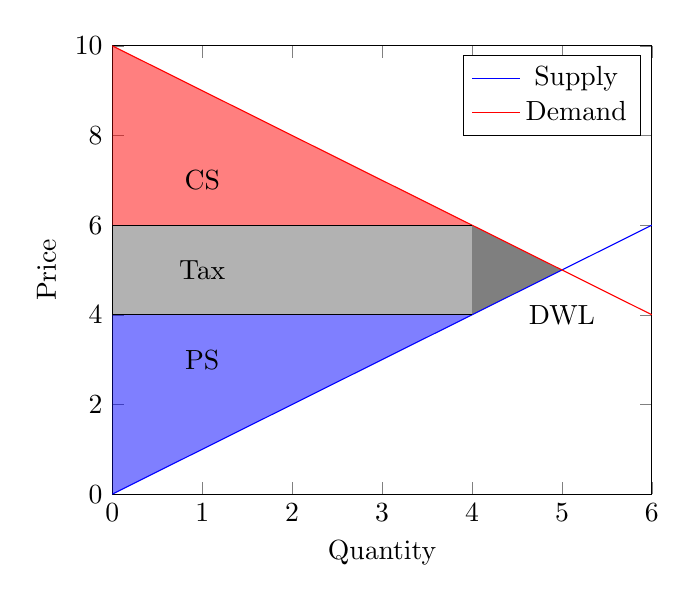
\begin{tikzpicture}
    \begin{axis} [
      xlabel={Quantity},
      ylabel={Price},
      xmin=0, xmax=6,
      ymin=0, ymax=10
    ]
      \addplot[name path=supply, color=blue] coordinates { (0,0) (6,6) };
      \addlegendentry{Supply};
      \addplot[name path=demand, color=red] coordinates { (0,10) (6,4) };
      \addlegendentry{Demand};
      \addplot[name path=tax1, color=black] coordinates { (0,4) (4,4) };
      \addplot[name path=tax2, color=black] coordinates { (0,6) (4,6) };
      \addplot[color=blue, fill=blue, fill opacity=0.5]
        fill between [of=tax1 and supply, soft clip={domain=0:4}];
      \addplot[color=red, fill=red, fill opacity=0.5]
        fill between [of=tax2 and demand, soft clip={domain=0:4}];
      \addplot[color=black, fill=black, fill opacity=0.3]
        fill between [of=tax1 and tax2, soft clip={domain=0:4}];
      \addplot[color=black, fill=black, fill opacity=0.5]
        fill between [of=supply and demand, soft clip={domain=4:5}];
      \node[draw=none] at (1,7) {CS};
      \node[draw=none] at (1,3) {PS};
      \node[draw=none] at (1,5) {Tax};
      \node[draw=none] at (5,4) {DWL};
    \end{axis}
  \end{tikzpicture}
\end{center}

\subsubsection{Practice Problem}
Brownies:
\begin{center}
  \begin{tabular}{|c|c|c|}
    \hline
    P       & \( Q_{D} \) & \( Q_{S} \) \\ \hline
    \$0.50  & 5           & 3           \\ \hline
    \$0.60  & 4           & 4           \\ \hline
    \$0.70  & 3           & 5           \\ \hline
    \$0.80  & 2           & 6           \\ \hline
    \$0.90  & 1           & 7           \\ \hline
  \end{tabular}
\end{center}
What is \( Q_{*} \) and \( P_{*} \) with no tax?
\[ P_{*} = 0.60 \quad Q_{*} = 4 \]
If sellers are taxed \$0.10 per brownie and buyers taxed \$0.10 per brownie,
then the price paid is \$0.70 per brownie and the price received is \$0.50 per
brownie. The quantity demanded and supplied is 3.

\subsection{Subsidies}
A subsidy is a payment made by the government to a producer, or a consumer.
A subsidy has the opposite effect of a tax.

\subsubsection{Example}
Suppose there is a \$20 subsidy to sellers:
\begin{center}
  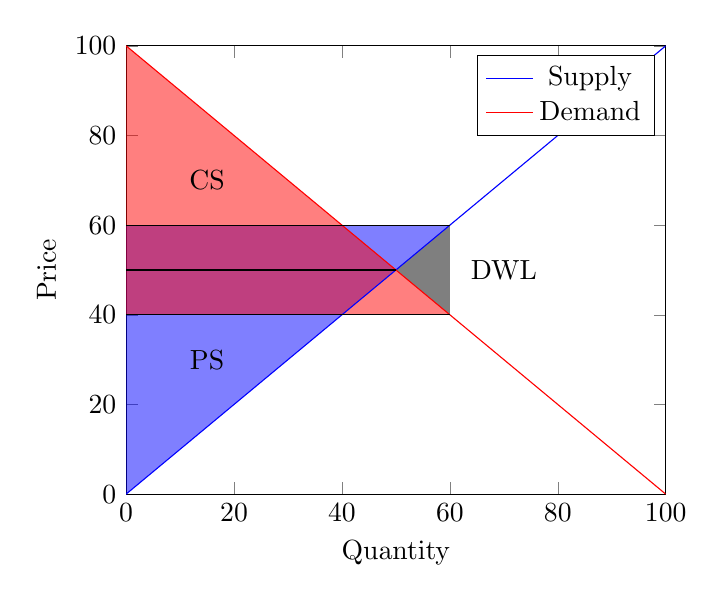
\begin{tikzpicture}
    \begin{axis} [
      xlabel={Quantity},
      ylabel={Price},
      xmin=0, xmax=100,
      ymin=0, ymax=100
    ]
      \addplot[name path=supply, color=blue] coordinates { (0,0) (100,100) };
      \addlegendentry{Supply};
      \addplot[name path=demand, color=red] coordinates { (0,100) (100,0) };
      \addlegendentry{Demand};
      \addplot[name path=subsidy1, color=black] coordinates { (0,60) (60,60) };
      \addplot[name path=subsidy2, color=black] coordinates { (0,40) (60,40) };
      \addplot[name path=split, color=black] coordinates { (0,50) (50,50) };
      \addplot[color=blue, fill=blue, fill opacity=0.5]
        fill between [of=subsidy1 and supply, soft clip={domain=0:60}];
      \addplot[color=red, fill=red, fill opacity=0.5]
        fill between [of=subsidy2 and demand, soft clip={domain=0:60}];
      \addplot[color=black, fill=black, fill opacity=0.5]
        fill between [of=supply and demand, soft clip={domain=50:60}];
      \node[draw=none] at (15,70) {CS};
      \node[draw=none] at (15,30) {PS};
      \node[draw=none] at (70,50) {DWL};
    \end{axis}
  \end{tikzpicture}
\end{center}
The consumer surplus and producer surplus both increase by 550. The cost of the
policy is 1200 (the rectangular region including the surpluses and the
dead-weight loss), so the total surplus decreases. \par
If a \$10 tax is imposed on buyers and a \$10 subsidy is imposed on sellers,
both curve shifts cancel and there is no net effect.

\subsubsection{Consequences of Subsidies}
\begin{itemize}
  \item Increases in supply
  \item Decrease in price
  \item Inefficient overproduction
  \item Consumer surplus and producer surplus increase
  \item Increases in surplus are offset by the cost of the subsidy, resulting in
  deadweight loss
\end{itemize}

\subsection{Production Quotas}
A production quota is an upper limit on the amount of a good that can be
produced. It is usually intended to help producers by raising prices.

\subsubsection{Consequences of a Production Quota}
\begin{itemize}
  \item Increase in price
  \item Decrease in consumer surplus
  \item Increase in producer surplus
  \item Transfer of surplus from consumers to producers
  \item Deadweight loss
  \item Provides an incentive for producers to cheat and overproduce
\end{itemize}

\subsection{Markets for Illegal Goods}
If illegal goods are taxed, it raises tax revenue for the government. On the
other hand, the government profits from the trade of harmful substances.
Formerly illegal drugs are now legitimate and thus might influence the
preferences of consumers.

\section{Global Markets}
International trade is driven by comparative advantages. A nation has a
comparative advantage in producing a good if it can produce it at a lower
opportunity cost than any other nation.

\subsection{Markets with Imports}
If the world price is less than the domestic equilibrium price, imports will
occur. Domestic consumers benefit from this while producers are harmed by this.
However, there is a net gain.

\subsection{Markets with Exports}
If the world price is greater than the domestic equilibrium price, exports will
occur. Domestic consumers are harmed by this while producers benefit from this.
There is a net gain overall.

\subsection{Protecting Domestic Producers: Trade Restrictions}

\subsubsection{Tariffs}
A tariff is a tax imposed on imports by the importing country. For example,
India imposes a 100\% tariff on wine imported from California. Domestic
producers benefit from import tariffs while consumers are worse off. The
government gains tariff revenue, but there is a still a deadweight loss
because consumers lose more than the amount gained by producers and the
government.

\subsubsection{Import Quotas}
An import quota is a limit on the quantity that can be imported. For example,
the US imports quotas on dairy products, chocolate, cotton, and brooms.
Domestic producers benefit from import quotas while domestic producers are
worse off. Importers gain profit, but there is still a deadweight loss because
consumers lose more than the amount gained by producers and the government.

\subsubsection{A Comparison of Tariffs and Quotas}
Given a desired level of imports, the same price is paid by consumers, the same
quantity is traded, the same amount of produced by domestic suppliers, and there
is the same deadweight loss. With tariffs, the government gains revenue, while
with quotas, importers gain profit.

\subsubsection{Example}
\[ Q_{supplied\ domestic} = P \]
\[ Q_{demanded\ domestic} = 10-P \]
\[ P_{world} = 2 \]
\begin{center}
  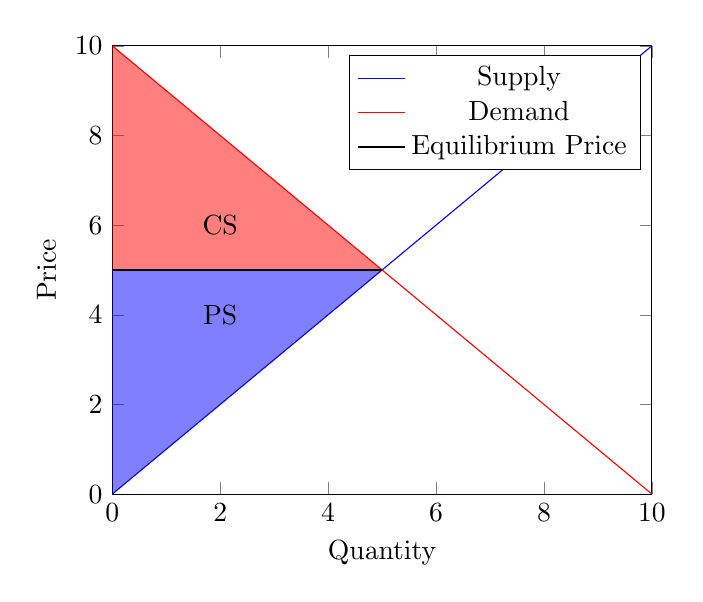
\begin{tikzpicture}
    \begin{axis} [
      xlabel={Quantity},
      ylabel={Price},
      xmin=0, xmax=10,
      ymin=0, ymax=10
    ]
      \addplot[name path=supply, color=blue] coordinates { (0,0) (10,10) };
      \addlegendentry{Supply};
      \addplot[name path=demand, color=red] coordinates { (0,10) (10,0) };
      \addlegendentry{Demand};
      \addplot[name path=equilibrium, color=black] coordinates { (0,5) (5,5) };
      \addlegendentry{Equilibrium Price};
      \addplot[color=blue, fill=blue, fill opacity=0.5]
        fill between [of=equilibrium and supply, soft clip={domain=0:5}];
      \addplot[color=red, fill=red, fill opacity=0.5]
        fill between [of=equilibrium and demand, soft clip={domain=0:5}];
      \node[draw=none] at (2,6) {CS};
      \node[draw=none] at (2,4) {PS};
    \end{axis}
  \end{tikzpicture}
\end{center}
\[ P^{*} = 10-P^{*} \]
\[ P^{*} = 5\ (\mathrm{equilibrium\ price}) \]
\begin{center}
  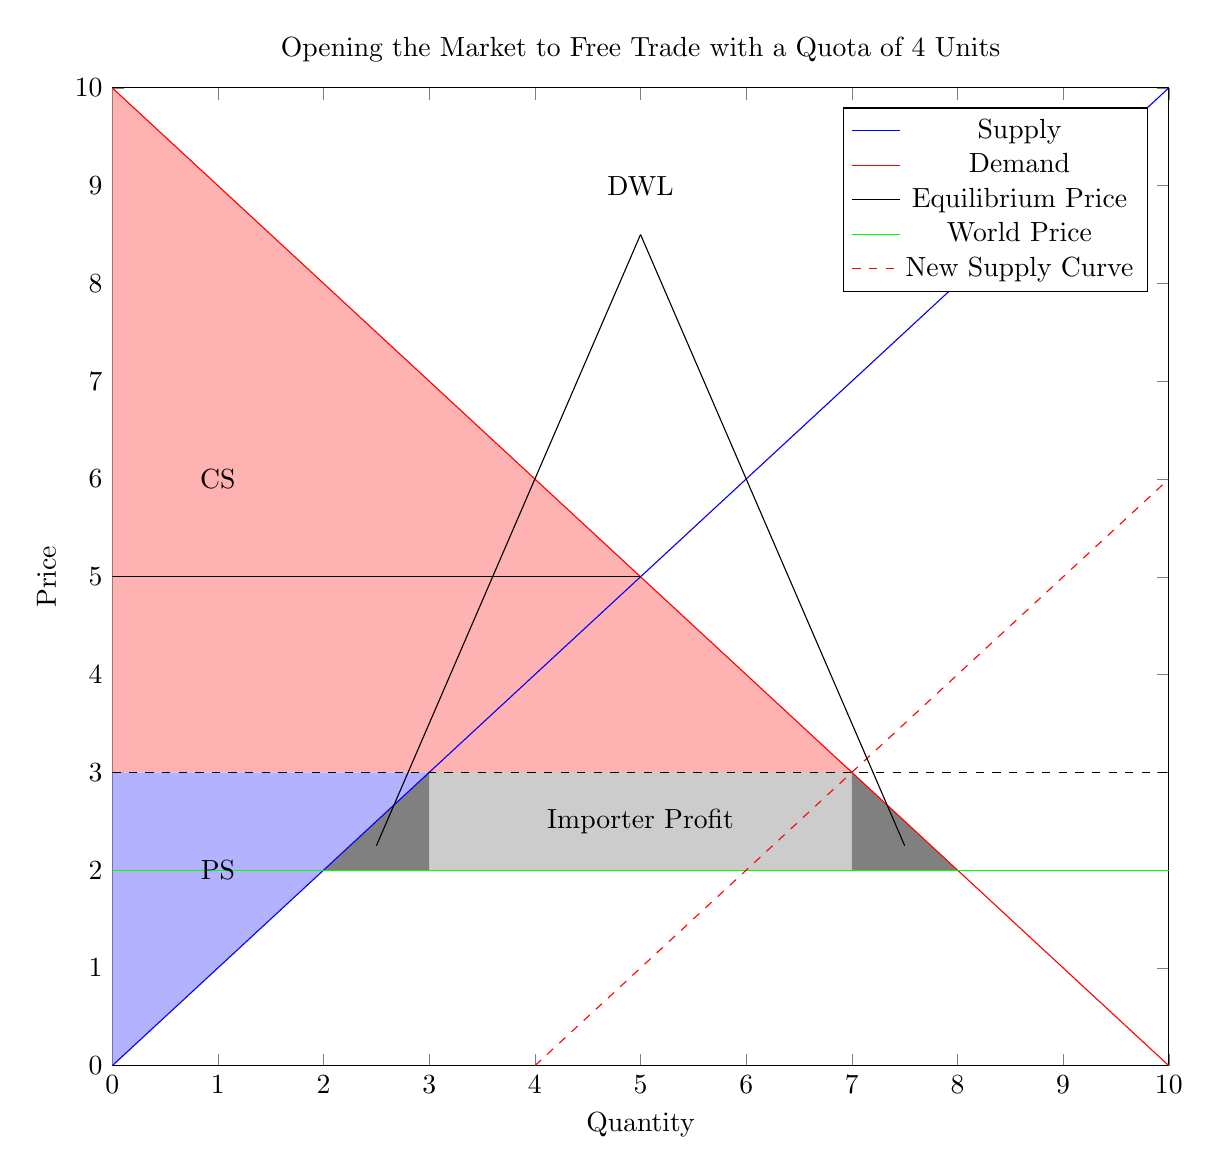
\begin{tikzpicture}
    \begin{axis} [
      xlabel={Quantity},
      ylabel={Price},
      width=15cm,
      height=14cm,
      title={Opening the Market to Free Trade with a Quota of 4 Units},
      xtick={0,1,...,10},
      ytick={0,1,...,10},
      xmin=0, xmax=10,
      ymin=0, ymax=10
    ]
      \addplot[name path=supply, color=blue] coordinates { (0,0) (10,10) };
      \addlegendentry{Supply};
      \addplot[name path=demand, color=red] coordinates { (0,10) (10,0) };
      \addlegendentry{Demand};
      \addplot[name path=equilibrium, color=black] coordinates { (0,5) (5,5) };
      \addlegendentry{Equilibrium Price};
      \addplot[name path=world, color=green] coordinates { (0,2) (10,2) };
      \addlegendentry{World Price};
      \addplot[name path=supply2, color=red, dashed] coordinates
        { (4,0) (10,6) };
      \addlegendentry{New Supply Curve};
      \addplot[name path=equilibrium2, dashed] coordinates { (0,3) (10,3) };
      \addplot[color=blue, fill=blue!30]
        fill between [of=equilibrium2 and supply, soft clip={domain=0:3}];
      \addplot[color=red, fill=red!30]
        fill between [of=equilibrium2 and demand, soft clip={domain=0:7}];
      \addplot[color=black, fill=black!20]
        fill between [of=equilibrium2 and world, soft clip={domain=3:7}];
      \addplot[color=black, fill=black!50]
        fill between [of=world and supply, soft clip={domain=2:3}];
      \addplot[color=black, fill=black!50]
        fill between [of=world and demand, soft clip={domain=7:8}];
      \node[draw=none] at (1,6) {CS};
      \node[draw=none] at (1,2) {PS};
      \node at (5,9) {DWL};
      \addplot[color=black] coordinates { (2.5,2.25) (5,8.5) };
      \addplot[color=black] coordinates { (7.5,2.25) (5,8.5) };
      \node[draw=none] at (5,2.5) {Importer Profit};
    \end{axis}
  \end{tikzpicture}
\end{center}
\[ 4 + P^{**} = 10-P^{**} \]
\[ 2P^{**} = 6 \]
\[ P^{**} = 3 \]

\subsection{Common Arguments For/Against Trade Restrictions}
\begin{itemize}
  \item Argument: They help infant industries grow.
  \item Counter-argument: They also protect firms that are not producing
  efficiently.
  \item Argument: They counteract dumping.
  \item Counter-argument: Dumping is very hard to detect because it
  is hard to know a firm's costs. A low price might be set by a producer
  because she faces elastic demand.
  \item Argument: They save domestic jobs.
  \item Counter-argument: They might create jobs in one sector and destroy
  jobs in another.
  \item Argument: They allow us to compete with cheap foreign labor.
  \item Counter-argument: Wages are determined by productivity. High
  productivity workers get higher wages and low productivity workers get lower
  wages.
  \item Argument: They protect rich countries from exploiting poor ones.
  \item Counter-argument: By trading with poor countries, we increase the
  demand for their labor and increase their income.
\end{itemize}

\section{Utility and Demand}
What determines the choices made by a consumer? Where do individual's demand
curves come from? Consumption Possibilities are determined by prices and
income.

\subsection{The Budget Line}
The \textbf{budget line} is the boundary between combinations that an
individual can afford and those that the individual cannot afford. The budget
line is determined by income and prices.

\subsubsection{Preferences and Utility}
Preferences describe an individual's likes and dislikes and how they rank
various bundles of goods. \textbf{Total Utility} is the total benefit or
satisfaction that a person gets from consuming goods. \textbf{Marginal
Utility} is the change in total utility that results from a one unit
increase in the quantity of a good consumed. The Consumer's Problem is to
choose the most preferred bundle among those she can afford, or, to choose
the bundle that gives her the highest utility among those she can afford.
An indifference curve describes all the consumption bundles among which
a consumer is indifferent.

\subsubsection{The Consumer's Problem}
Given some transitive relationship \( X>Y \), \( X<Y \), or \( X\sim Y \),
there exists a function \( u(x,y) \) which yields the total utility of the
goods. The problem is reduced to maximizing \( u(x,y) \). The consumer
chooses a bundle that maximizes utility within the constraints. \par
We will assume positive marginal utility, which means that more is always
better. We will also assume diminishing marginal utility, which means the
increase in utility is smaller the greater the quantity of the good. The
goal is to find the preferred bundle on the budget line.
\begin{center}
  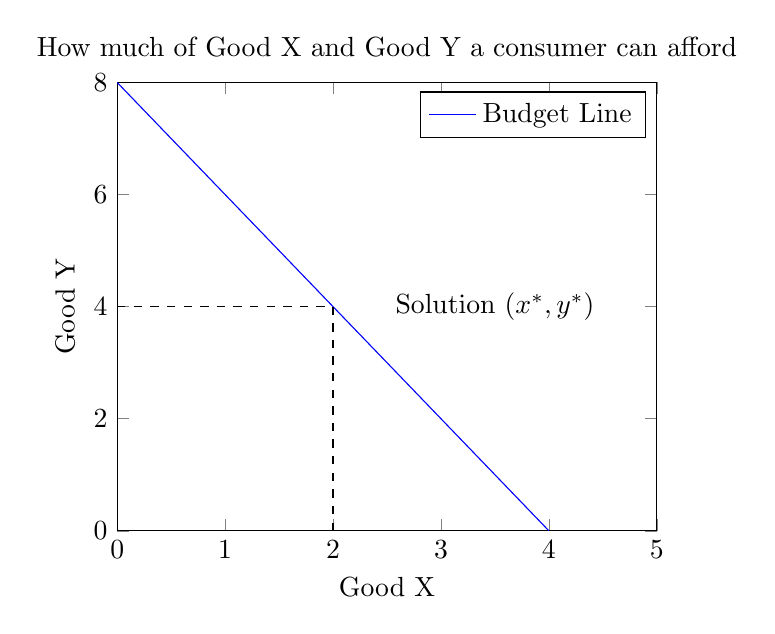
\begin{tikzpicture}
    \begin{axis} [
      xlabel={Good X},
      ylabel={Good Y},
      title={How much of Good X and Good Y a consumer can afford},
      xmin=0, xmax=5,
      ymin=0, ymax=8
    ]
      \addplot[name path=supply, color=blue] coordinates { (0,8) (4,0) };
      \addlegendentry{Budget Line};
      \addplot[dashed, color=black] coordinates { (2,0) (2,4) };
      \addplot[dashed, color=black] coordinates { (0,4) (2,4) };
      \node[draw=none] at (3.5,4) {Solution \( (x^{*},y^{*}) \)};
    \end{axis}
  \end{tikzpicture}
\end{center}
\[ p_{x}x^{*}+p_{y}y^{*} = m \]
\[ u(x,y) = u_{x}(x)+u_{y}(y) \]
\[ \frac{mu_{x}(x^{*},y^{*})}{p_{x}} = \frac{mu_{y}(x^{*},y^{*})}{p_{y}} \]

\subsubsection{Example}
\[ m = 40 \quad p_{x} = 8 \quad p_{y} = 4 \]
\begin{center}
  \begin{tabular}{|c|c|c|c|}
    \hline
    \( x \) & \( u_{x} \) & \(y \) & \( u_{y} \) \\ \hline
    0       & 0           & 0      & 0           \\ \hline
    1       & 50          & 1      & 25          \\ \hline
    2       & 90          & 2      & 123         \\ \hline
    3       & 122         & 3      & 159         \\ \hline
    4       & 150         & 4      & 183         \\ \hline
    5       & 176         & 5      & 205         \\ \hline
    6       & 200         & 6      & 225         \\ \hline
    7       & 222         & 7      & 238         \\ \hline
    8       & 242         & 8      & 243         \\ \hline
    9       & 259         & 9      & 255         \\ \hline
    10      & 295         & 10     & 260         \\ \hline
  \end{tabular}
\end{center}
Find (x,y) on the budget line, and find the bundle on the budget line that
gives the highest utility:
\begin{center}
  \begin{tabular}{|c|c|c|c|c|}
    \hline
    \( x \) & \( y \) & \( u_{x} \) & \( u_{y} \) & \( u(x,y) \) \\ \hline
    0       & 10      & 0           & 260         & 260          \\ \hline
    1       & 8       & 50          & 248         & 298          \\ \hline
    2       & 6       & 90          & 225         & 315          \\ \hline
    3       & 4       & 122         & 183         & 305          \\ \hline
    4       & 2       & 150         & 123         & 273          \\ \hline
    5       & 0       & 176         & 0           & 176          \\ \hline
  \end{tabular}
\end{center}
\( u(x,y) \) is maximized at (2,6).

\section{Key Terms and Ideas}
\textbf{Absolute Advantage (AA)}: A person (or country) has an absolute
advantage if they are more productive than others.
\newline
\textbf{Allocative Efficiency}: An allocation of goods that maximizes benefit
(total benefit - total cost).
\newline
\textbf{Comparative Advantage (CA)}: A person (or country) has a comparative
advantage in an activity if they can perform that activity at a lower
opportunity cost that everyone else.
\newline
\textbf{Demand}: The entire relationship between the price of a good and the
quantity demanded of that good.
\newline
\textbf{Diminishing Marginal Benefit}: The more of a good an individual has,
the less the individual is willing to give up for one more unit of that good.
\newline
\textbf{Function}: The relationship between two quantities.
\newline
\textbf{Gains From Trade}: The net benefit to agents who conduct trade of
specific goods.
\newline
\textbf{Marginals}: The variance in the output of a function as the input value
changes by a given amount. Analogous to the derivative of a function.
\newline
\textbf{Marginal Benefit}: The total amount of a good that an individual is
willing to give up for ONE unit of another good.
\newline
\textbf{Marginal Cost}: The opportunity cost of producing one additional unit
of some good. Ex: ``I give up 3 cookies to produce the 6th unit of cat food''.
\newline
\textbf{Marginal Utility}: The change in total utility that results from a
one unit increase in the quantity of a good consumed.
\newline
\textbf{Minimum Wage}: A government regulation making it illegal to pay a
worker less than a specified wage.
\newline
\textbf{Normative Statement}: An expression of how things ought to be.
\newline
\textbf{Opportunity Cost (OC)}: The highest valued alternative for the action.
\newline
\textbf{Pareto Efficiency}: An allocation is pareto efficient if there is no
way to make an individual better off without making someone else worse off.
\newline
\textbf{Positive Statement}: An expression of how things are.
\newline
\textbf{Price Ceiling}: A regulation making it illegal to charge more than
a specified price.
\newline
\textbf{Price Elasticity of Demand}: A measure of the responsiveness of the
demand for a good to a change in its \textit{price}, ceteris paribus.
\newline
\textbf{Price Floor}: A regulation making it illegal to charge less than
a specified price.
\newline
\textbf{Production Efficiency}: Goods are produced at the lowest possible
opportunity cost.
\newline
\textbf{Production Possibilities Frontier (PPF)}: The set of all possible goods
that can be produced at a given point in time.
\newline
\textbf{Subsidies}: A payment made by the government to a producer or a
consumer.
\newline
\textbf{Supply}: The entire relationship between the quantity supplied of a
good and its price.
\newline
\textbf{Tax}: A levy imposed on an individual or legal entity by the state
whose failure to be paid can be punishable by law.
\newline
\textbf{Tax Incidence}: The division of the burden of a tax between buyers and
sellers.
\newline
\textbf{Total Benefit}: The total amount of a good that an individual is
willing to give up for some amount of another good.
\newline
\textbf{Total Revenue}: The price of a good times the quantity sold.
\newline
\textbf{Total Utility}: The total benefit or satisfaction a person gets from
consuming goods.

\begin{center}
  If any errors are found, please contact me at alvin.lin.dev@gmail.com
\end{center}

\end{document}
